\documentclass[conference]{IEEEtran}

% Language setting
% Replace `english' with e.g. `spanish' to change the document language
\usepackage[english]{babel}

% Useful packages
\usepackage{amsmath}
\usepackage{graphicx}
\usepackage{url}

% Title and author info
\title{GuitarHero Prototype}
\author{\IEEEauthorblockN{Juan David Cotacio Sánchez}}

\begin{document}
\maketitle

\begin{abstract}
Your abstract.
\end{abstract}

\section{Introducción}
En este emocionante proyecto, exploraremos cómo recrear la experiencia única de tocar una guitarra en un videojuego clásico como Guitar Hero, ¡todo dentro de tu navegador web! Utilizaremos tecnologías web fundamentales como HTML, CSS y JavaScript para construir nuestro prototipo.





\subsection{Como empezar el prototipo}

Para la creación de este prototipo empece en como podia implementar estas tres tecnologias, para la inclusión de esta herramientas empece por crear un HTML y CSS a la vez, para poder darle un espacio en mi pagina web y un estilo para que sea agradable a la vista.
\begin{figure}[h] % Aquí comienza la inclusión de la imagen
    \centering
    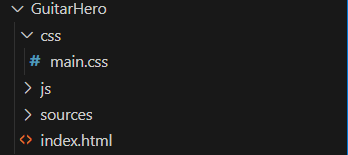
\includegraphics[width=0.5\textwidth]{Guitar Hero One.png} % Reemplaza 'ruta/de/la/imagen' por la ruta de tu imagen
    \caption{Creación de CSS y HTML}
    \label{fig:mi_imagen}
\end{figure}

\subsection{Como se incluyo el CSS y HTML}
Primero empece a crear una estructura en mi HTML para darle el espacio, cree un contenedor general que iba almacenar mis notas musicales, mastil, cuerdas, hitters, botones y background.

En mi css quise añadir las respectivas imagenes de cada una de las cosas que estaba añadiendo en mi HTML, para darle posición, tamaños y animaciónes.Unas de las cosas más complejas fue darle una animación a mis notas y fondo del mastil, pues en una investigación encontre que el @Keyframes se puede usar para poder darle un movimiento desde mi CSS.

\begin{figure}[h] % Aquí comienza la inclusión de la imagen
    \centering
    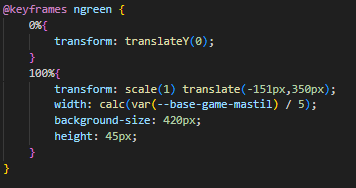
\includegraphics[width=0.5\textwidth]{KeyFrames.png} % Reemplaza 'ruta/de/la/imagen' por la ruta de tu imagen
    \caption{Uso del KeyFrames}
    \label{fig:mi_imagen}
\end{figure}



\subsection{Implementación Java Script}

Para la implementación del JS en este prototipo fue principalmente para añadir eventos al click, teclas, configuracion de la aparición de teclas de forma aleatoria, la desaparición de las notas y la introducción de musica al prototipo.

Una de la cosas complejas fue el hecho de configurar el "collider"
para las notas desaparecieran al momento de que el usuario oprimiera la teclas correcta o incorrecta, pues se tenia que implementar 

\begin{figure}[h] % Aquí comienza la inclusión de la imagen
    \centering
    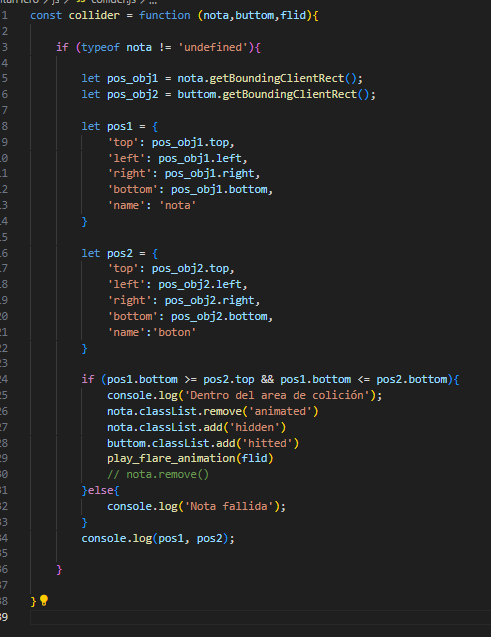
\includegraphics[width=0.3\textwidth]{collider.png} % Reemplaza 'ruta/de/la/imagen' por la ruta de tu imagen
    \caption{Collider en JavaScript}
    \label{fig:mi_imagen}
\end{figure}


\subsection{Pruebas del Prototipo}

Por último faltaria importar la logica a mi HTML para que esta pueda correr de manera secuencial y adecuada para lo que seria un Guitar Hero cabe recalcar que tambien se importo la hoja de estilos una parte importante de este proyecto.

Una de las cosas más complejas fue solucinar el problema de la privacidad y seguridad de los navegadores, pues estos no dejan repoducir multimedia por estas mismas razones, una de las manera para solucionarlo fue la instalación de uan extensión de Visual Studio, LifeServer gracias a esta extension la musica puede reproducirse.

\begin{figure}[h] % Aquí comienza la inclusión de la imagen
    \centering
    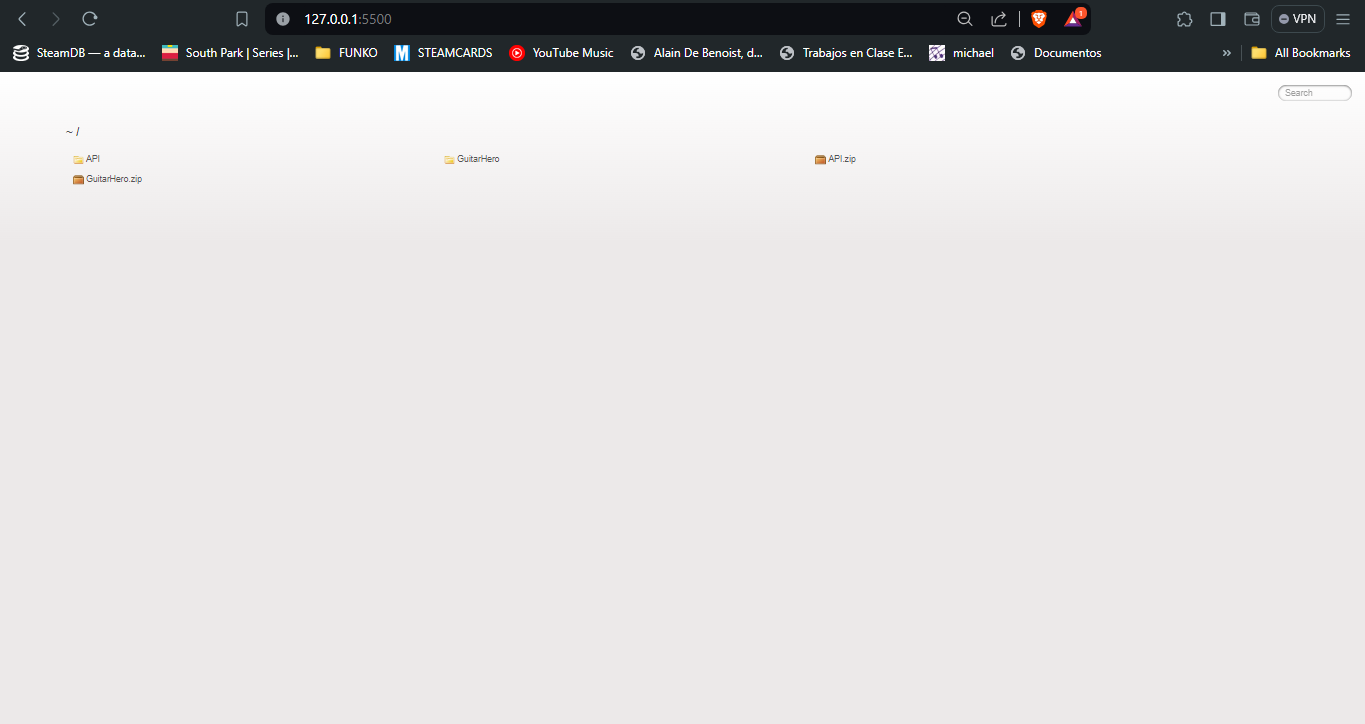
\includegraphics[width=0.5\textwidth]{Life server.png} % Reemplaza 'ruta/de/la/imagen' por la ruta de tu imagen
    \caption{Uso de lifeserver}
    \label{fig:mi_imagen}
\end{figure}

\subsection{Vista General del Prototipo}
En la vista general de mi protipo se trato de llegar a lo más similar de un GuitarHero manteniendo las esencia original del videojuego, además de hacerlo funcional, como se podran mostrar en las siguientes figuras.

\begin{figure}[h] % Aquí comienza la inclusión de la imagen
    \centering
    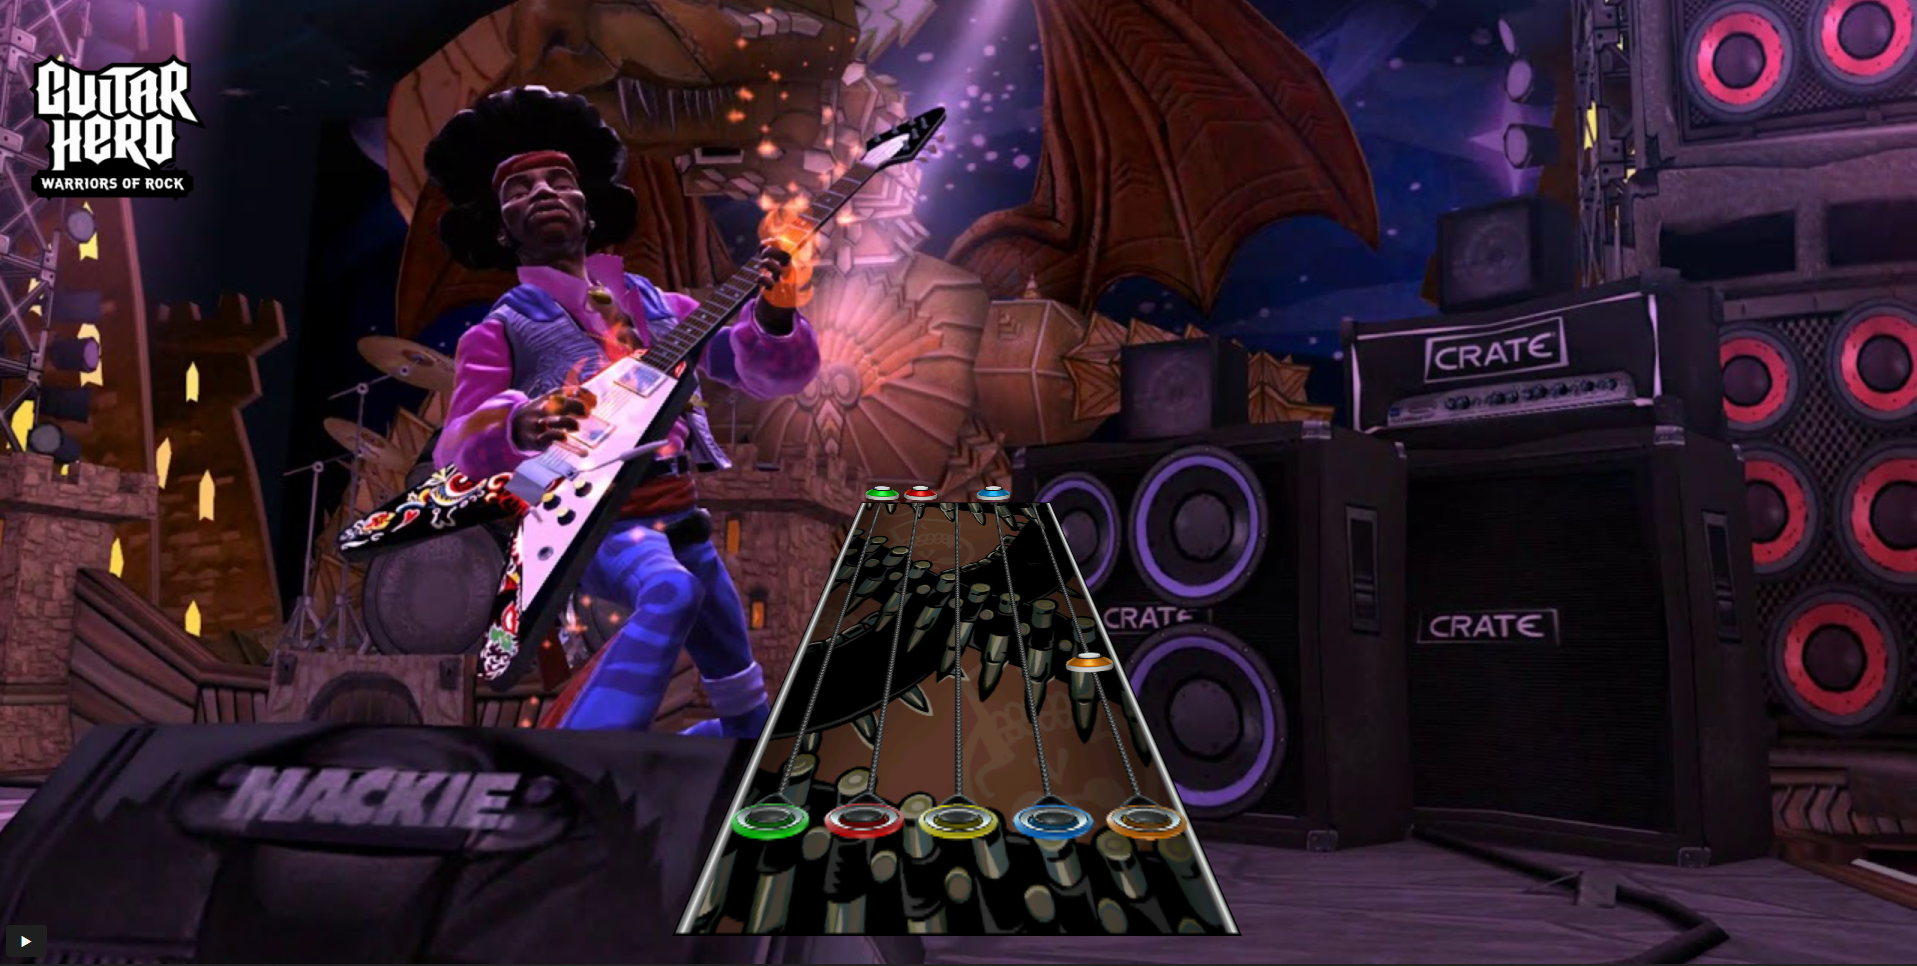
\includegraphics[width=0.5\textwidth]{GuitarHeroView.png} % Reemplaza 'ruta/de/la/imagen' por la ruta de tu imagen
    \caption{Vista Final Del Prototipo}
    \label{fig:mi_imagen}
\end{figure}

\subsection{Instructivo}
Para que el juego se pueda disfrutar en terminos general se debe ajustar siempre valores, para que el contenido se adapte a la pantalla y no se vea desproporcioando se pued eutilizar la combinacion de teclas "ctrl + +" o en su defecto "ctrl + -", estos valores son adaptables al gusto del usuario pero para resoluciones 1920 x 1080, el 90 prociento queda perfectamente ancajado.

Para la musica se necesita ajustar el volumen a preferencia del usuario pues puede arruinar la experencia del juego, entonces estos valores son adaptables al gusto del usuario usando la funciones que se brinda en el navegador y OS
\begin{figure}[h] % Aquí comienza la inclusión de la imagen
    \centering
    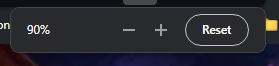
\includegraphics[width=0.5\textwidth]{Zoom.png} % Reemplaza 'ruta/de/la/imagen' por la ruta de tu imagen
    \caption{Zoom para resoluciones 1920 x 1080}
    \label{fig:mi_imagen}
\end{figure}

\begin{figure}[h] % Aquí comienza la inclusión de la imagen
    \centering
    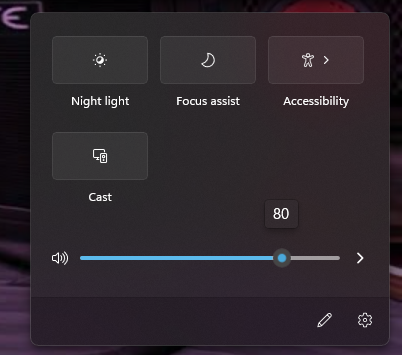
\includegraphics[width=0.4\textwidth]{Volume.png} % Reemplaza 'ruta/de/la/imagen' por la ruta de tu imagen
    \caption{Volumen recomendado}
    \label{fig:mi_imagen}
    \vspace{500pt} % Ajusta el espacio vertical aquí según tus necesidades
\end{figure}
\end{document}

